\documentclass[a4paper,12pt]{article}
\usepackage[utf8]{inputenc}
\usepackage{graphicx}
\usepackage{float}
\usepackage{listings}
\usepackage{courier}

\usepackage{xcolor}
\definecolor{gris}{RGB}{123, 126, 132}
\definecolor{morado}{RGB}{81, 40, 155}
\definecolor{amarillo}{RGB}{253,151,31}
\definecolor{magenta}{RGB}{249,38,114}

\renewcommand{\lstlistingname}{Archivo}

\lstdefinestyle{customXML}{
    frame=tb,
    language=XML,
    basicstyle=\footnotesize\ttfamily,
    backgroundcolor=\color{white},   
    commentstyle=\itshape\color{gris},
    keywordstyle=\bfseries\color{magenta},
    numberstyle=\color{morado},
    stringstyle=\color{amarillo},
    identifierstyle=\color{morado},
    basicstyle=\footnotesize,
    breakatwhitespace=false,         
    breaklines=true,                 
    captionpos=b,
    keepspaces=true,                 
    numbers=left,                    
    numbersep=5pt,                  
    showspaces=false,                
    showstringspaces=false,
    showtabs=false,                  
    tabsize=2,
    morekeywords={web-app, encoding, xmlns, xmlns:xsi, xsi:schemaLocation}
}

\lstdefinestyle{customHTML}{
    frame=tb,
    language=HTML,
    basicstyle=\footnotesize\ttfamily,
    backgroundcolor=\color{white},   
    commentstyle=\itshape\color{gris},
    keywordstyle=\bfseries\color{magenta},
    numberstyle=\color{morado},
    stringstyle=\color{amarillo},
    identifierstyle=\color{morado},
    basicstyle=\footnotesize,
    breakatwhitespace=false,         
    breaklines=true,                 
    captionpos=b,
    keepspaces=true,                 
    numbers=left,                    
    numbersep=5pt,                  
    showspaces=false,                
    showstringspaces=false,
    showtabs=false,                  
    tabsize=2,
}

%opening
\title{Ejercicio No. 1. Despliegue de aplicación en Apache Tomcat}
\author{Barrera Pérez Carlos Tonatihu \\ Profesor: José Asunción Enríquez 
Zárate 
\\ Web Application Development \\ Grupo: 3CM9 }

\begin{document}

\maketitle
\newpage
\tableofcontents
\newpage

\section{Introducción}
\section{Desarrollo}
Para poder realizar este ejercicio lo primero que se hizo fue crear la 
siguiente estructura del proyecto.

\begin{figure}[H]
\begin{center}
 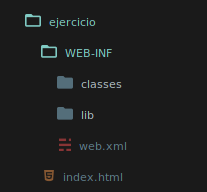
\includegraphics[width=6cm]{estructura.png}
 % estructura.png: 800x436 px, 96dpi, 21.16x11.53 cm, bb=0 0 600 327
 \caption{Estructura del proyecto}
 \label{fig:estructura}
\end{center}
\end{figure}

Lo siguiente fue crear los archivos index.html y web.xml con el siguiente 
contenido.

\begin{lstlisting}[language=XML, style=customXML, 
caption={web.xml},captionpos=b]
<?xml version="1.0" encoding="UTF-8"?>
<web-app version="3.0" xmlns="http://java.sun.com/xml/ns/javaee" 
xmlns:xsi="http://www.w3.org/2001/XMLSchema-instance" 
xsi:schemaLocation="http://java.sun.com/xml/ns/javaee 
http://java.sun.com/xml/ns/javaee/web-app_3_0.xsd">
    <display-name>Ejercicio 1</display-name>
    <servlet>
        <servlet-name>index</servlet-name>
        <jsp-file>/index.html</jsp-file>
    </servlet>
    <servlet-mapping>
        <servlet-name>index</servlet-name>
        <url-pattern>/index</url-pattern>
    </servlet-mapping>
</web-app>
\end{lstlisting}

\begin{lstlisting}[language=C, style=customHTML, 
caption={index.html},captionpos=b]
<!DOCTYPE html>
<html lang="es">
<head>
    <meta charset="UTF-8">
    <title>Ejercicio 1</title>
</head>
<body>
    <h1>Este es el ejercicio 1</h1>
    <h2>Que onda que pex</h2>
</body>
</html>
\end{lstlisting}

Después, se ejecuta el siguiente comando en la raíz del proyecto para poder 
generar un archivo .war.

\begin{figure}[H]
\begin{center}
 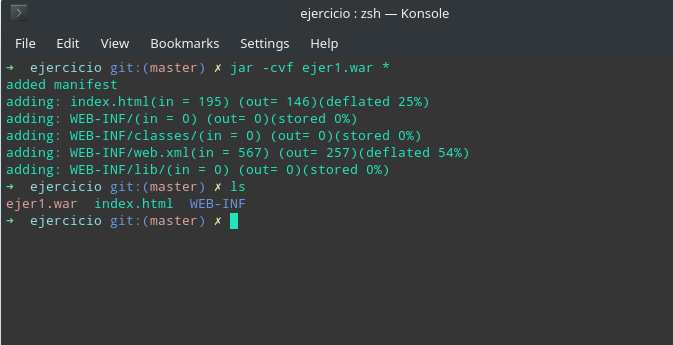
\includegraphics[width=12cm]{comando.png}
 % estructura.png: 800x436 px, 96dpi, 21.16x11.53 cm, bb=0 0 600 327
 \caption{Creación del archivo .war}
 \label{fig:comando}
\end{center}
\end{figure}

Lo siguiente es iniciar el Apache Tomcat ubicándonos en la carpeta /bin que se 
encuentra dentro de este contenedor web y ejecutar el siguiente comando.

\begin{figure}[H]
\begin{center}
 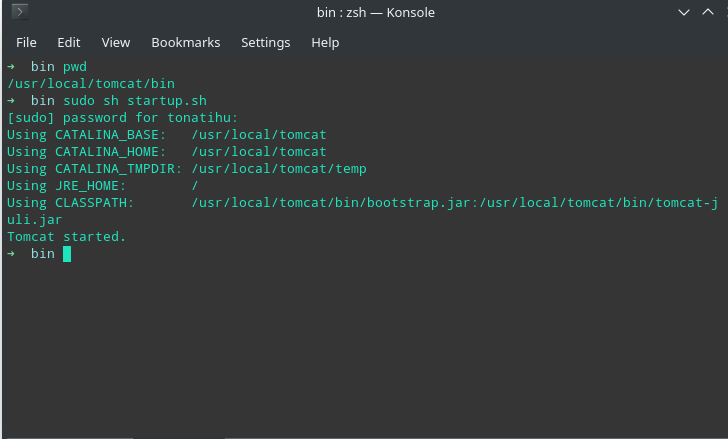
\includegraphics[width=12cm]{tomcat.png}
 % estructura.png: 800x436 px, 96dpi, 21.16x11.53 cm, bb=0 0 600 327
 \caption{Se inicia Apache Tomcat}
 \label{fig:tomcat}
\end{center}
\end{figure}

Vamos a la dirección localhost:8080 y entramos en la sección de gestión de 
aplicaciones y cargamos el archivo war generado anteriormente.

\begin{figure}[H]
\begin{center}
 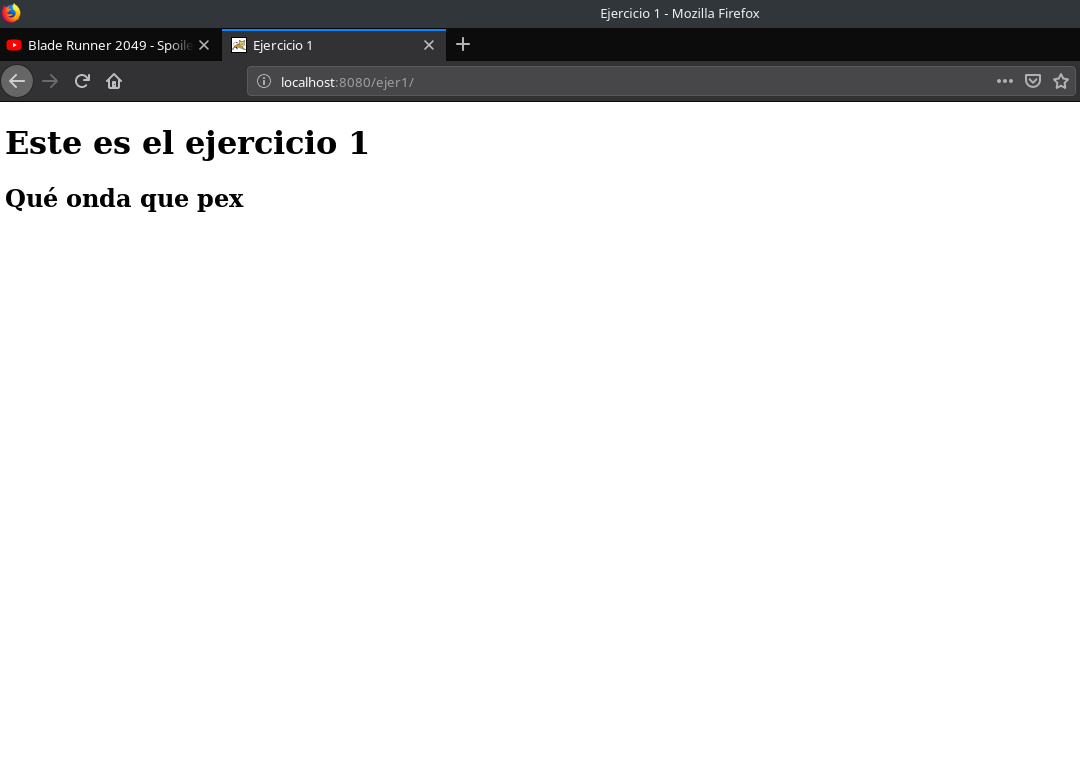
\includegraphics[width=12cm]{localhost.png}
 % estructura.png: 800x436 px, 96dpi, 21.16x11.53 cm, bb=0 0 600 327
 \caption{Pagina de inicio de Apache Tomcat}
 \label{fig:localhost}
\end{center}
\end{figure}

Y la pagina esta lista.

\begin{figure}[H]
\begin{center}
 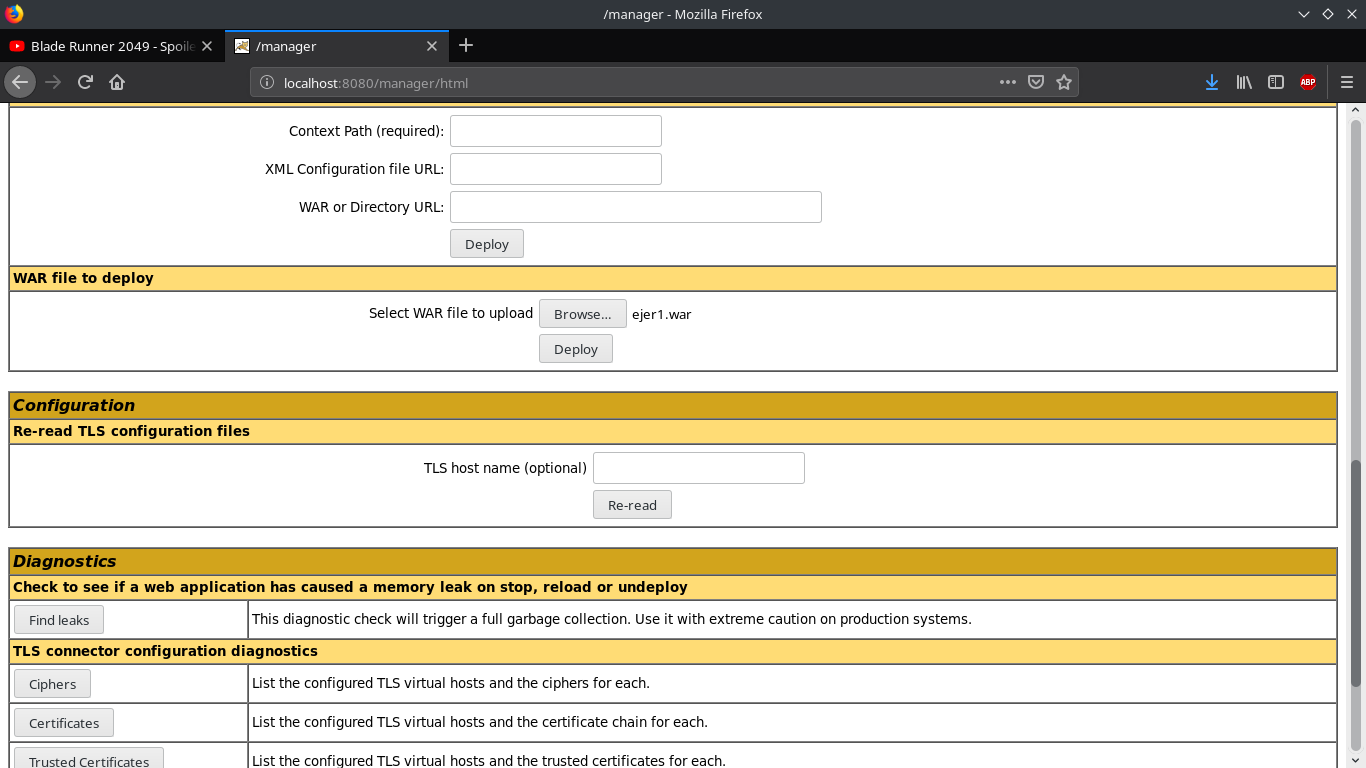
\includegraphics[width=12cm]{pagina.png}
 % estructura.png: 800x436 px, 96dpi, 21.16x11.53 cm, bb=0 0 600 327
 \caption{Index que se creo anteriormente}
 \label{fig:index}
\end{center}
\end{figure}

\section{Conclusiones}
Este ejercicio es un paso fundamental en el desarrollo de aplicaciones web, ya 
que el despliegue siempre se realiza en algún punto del desarrollo, y tal vez 
no siempre se utilice apache tomcat para esta tarea pero el conocer algo tan 
basico como esto siempre es útil.

\end{document}
